% geometry_and_trigonometry:x08 GDC:YES
\begin{question}
  \hspace*{\fill} [Note Maximale: 16]\par
  \medskip
  \begin{center} % or flushleft or flushright
    \noindent La figure ci-dessous représente le plan d'une fenêtre en forme de trapèze.\par
    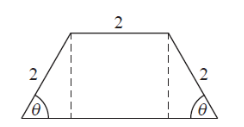
\includegraphics[scale=0.5]{figure_x8}\par
  \end{center} % or flushleft or flushright
  \noindent Trois côtés de la fenêtre ont une longueur de $2 m$. L'angle entre les côtés obliques de la fenêtre et la base est $\theta$, où $0 \le \theta \le \frac{\pi}{2}$.\par

  \begin{enumerate}[label=(\alph*)]
    \item Montrez que l'aire de la fenêtre est donnée par $y = 4\,sin\,\theta + 2\,sin\,2\theta$. \hspace*{\fill} [5]
    \item Zoé veut une fenêtre avec une aire de $5 m^2$. Trouvez les deux valeus possibles de $\theta$\hspace*{\fill} [4]
    \item John veut deux fenêtres qui ont la même aire $A$ mais des valeurs différentes de $\theta$. Trouvez toutes les valeurs possibles de $A$.\hspace*{\fill} [7]
  \end{enumerate}
\end{question}
